\documentclass[12pt,a4paper,titlepage]{article}
\usepackage[hmargin=2cm,vmargin=2.5cm]{geometry}
\usepackage[latin1]{inputenc}
\usepackage{amsmath}
\usepackage{amsfonts}
\usepackage{amssymb}
\usepackage{graphicx}
\usepackage{listings}
\usepackage{datetime}
\usepackage{url}
\usepackage[colorlinks=false]{hyperref}
\usepackage{gensymb}
\usepackage{subfigure}

\hypersetup{pdfborder = {0 0 0}}

\author{}
\title{Puma for FreeEMS\newline Assembly, configuration, modification and installation manual}

\begin{document}
\maketitle
\pagebreak

\tableofcontents
\thispagestyle{empty}
\pagebreak

\section{Overview}

This document is to show how to choose components to order, properly build and connect your Spin 1 board to a vehicle.

Puma uses FreeEMS vanilla firmware, PC tuning software and Puma hardware to control fuel and ignition of large variety of engine configurations. See \url{http://puma.freeems.org} for a more detailed overview of what PUMA can do and is used for.

We recommend you purchase the hardware such that many of the below steps aren't required. This version of the manual includes instructions for the Spin 1 board, which was generally provided as just a bare board. You will need to purchase parts based on a BOM then install those parts. You will also need to program the board via BDM programming port to get the initial bootloader installed. After the initial build, you will be able to program the board with an USB cable and a standard PC.

Note these sections are written as modules, such that sections are useful on their own, but also arranged in a sequence that is handy for a first time installer.

\section{Getting the hardware}

The design and software is OpenSource and while you can technically build it by yourself, we recommend you purchase PUMA assembled.

There are two ways to get an assembled board: sign up on forum.diyefi.org and ask for one, or go to \url{puma.freeems.org} and place an order.

Spin 1 was offered as a bare board, semi-assembled board, and a couple were fully assembled, so there are notes about how to do some low level assembly, but future spins will likely remove these assembly notes.

\section{So you have a bare board, now what?}

Ok, you have the bare PCB, and it's going to need components installed on it to function as a EMS. This is what you need to do, in no particular order:
\newline

Get the BOM from \url{https://github.com/nitrousnrg/puma/blob/master/BOMs/order_BOM.xls}, select which modules you need to have populated and the get the components.
\newline

For digikey custumers:

The third page is a digikey formatted file, ready to be saved as .csv to place the order.
\newline

For newark/mouser/farnell customers:

Use the MFG number to place your order, available in the second sheet, named ``MFG BOM''.



A few things to note:
\begin{itemize}
\item EGT circuit won't work, it has a 500$^{\circ}$C limit.
\item The usb connector is plain wrong. In the BOM you can choose to buy a cable to use this wrong (female-A) connector, or buy another usb connector and hack things to install it.
\item You don't want the shutdown circuit, so its FETs aren't in the BOM. Don't worry about that.
\end{itemize}

Once you are decided about the BOM, go to to digikey, mouser, newark or your favourite distributor and place the order.
\newline

\textbf{IMPORTANT:} If needed, modify the PCB as shown in ``Spin 1 specific notes''
\newline

We recommend doing these steps sequentially.

\begin{enumerate}
\item Install MCU and critical components.
\item Test the MCU works by uploading the firmware
\item Install rpm input circuit choose hall input, or VR
\item Install misc outputs like Fuel, ect
\item Install injectors circuits
\item Install ignitions circuits
\end{enumerate}


\subsection{You now have a PUMA board with components, now what?}

You will likely want to verify the board is good with a Jim Stim  then it will need the initial firmware installed. If PUMA was purchased assembled, these steps should not be required, and you can proceed to the next step.

\subsection{Testing your board with Jim Stim.}

Blah blah blah, fill in this stuff.

\subsection{Uploading the initial firmware.}

You need:
\begin{itemize}
\item A BDM programmer like TBDML, PE micros, etc.

Buy, borrow or build a BDM pod compatible with Freescale S12

This is an interesting one \url{http://www.flashgenie.net/USBDM.html}

\item CodeWarrior IDE or standalone app for code programming

Get the CodeWarrior IDE from (???), or download a small app from

\url{http://sourceforge.net/projects/usbdm/files/Version%204.5/1.%20Installation_4_5/USBDM_Win32_4_5.zip/download, check "HCS12_FlashProgrammer".}

\item A Serial Monitor binary

You can get the Serial monitor binary from the folowing url:
\newline

https://github.com/fredcooke/freeems-vanilla/raw/master/lib/freeems.serial.monitor.s19
\newline


\end{itemize}

Now proceed to the programming, the order is important:
\begin{enumerate}
\item Connect the BDM to the board
\item Connect the USB cable of the BDM to your PC
\item Supply Puma with 12v
\item Open Codewarrior's debugger, or execute directly

C:\textbackslash Archivos de programa\textbackslash Freescale\textbackslash CodeWarrior for HCS12 V4.7\textbackslash hiwave
\newline

The BDM pod should perform some recognition tasks
\item In the debugger, go to File-\textgreater Load Application and select the .s19 binary.

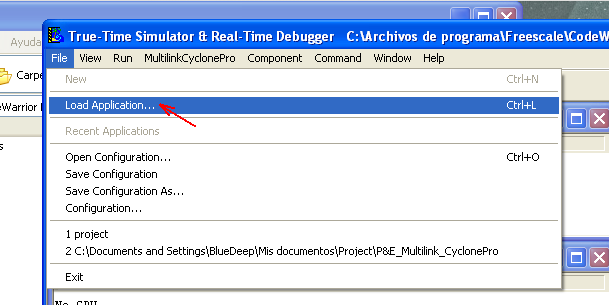
\includegraphics[width=0.9\textwidth]{images/CW_debugger_load.png}

\item Program the device. Verification should be successful.
\item Poweroff the board, then disconnect the USB, then disconnect the pod
\end{enumerate}

Now you can load the latest FreeEMS firmare!
\newline

Install SeanK's loader from https://github.com/seank/freeems-loader
\newline

Its an easy to use application. Just connect to the USB and power up Puma (jumpering the load/run header), select the device /dev/ttyUSB0 in *nixes (COM?? in windows?), and push the load button. In the file dialog, select the .s19 firmware you want. Wait until it erases and program the device.
Close the communications.

Remove the load/run jumper in the header and reset de board.

Congratulations! FreeEMS code is running in your board.

\section{Uploading firmware via USB and boot loader}

So you have a PUMA that may or may not be connected to your system.

This is how to upload a new firmware file to that board.

\begin{itemize}
\item Download and install

\item Open

\item Configure USB port

\item Specify to upload firmware file.
\end{itemize}


\section{Trying out the board with a Tuning Software}

Install and open Megatunix (from github link?). Select FreeEMS as the ECU system, and hit ''Find my ECU``.



\section{Connecting the board to a vehicle}

\subsection{The basics}
Figure~\ref{fig:wiring} shows how the PUMA board should be connected to the engine.

%I want this image *here*!
\begin{figure}[h!]
\begin{center}
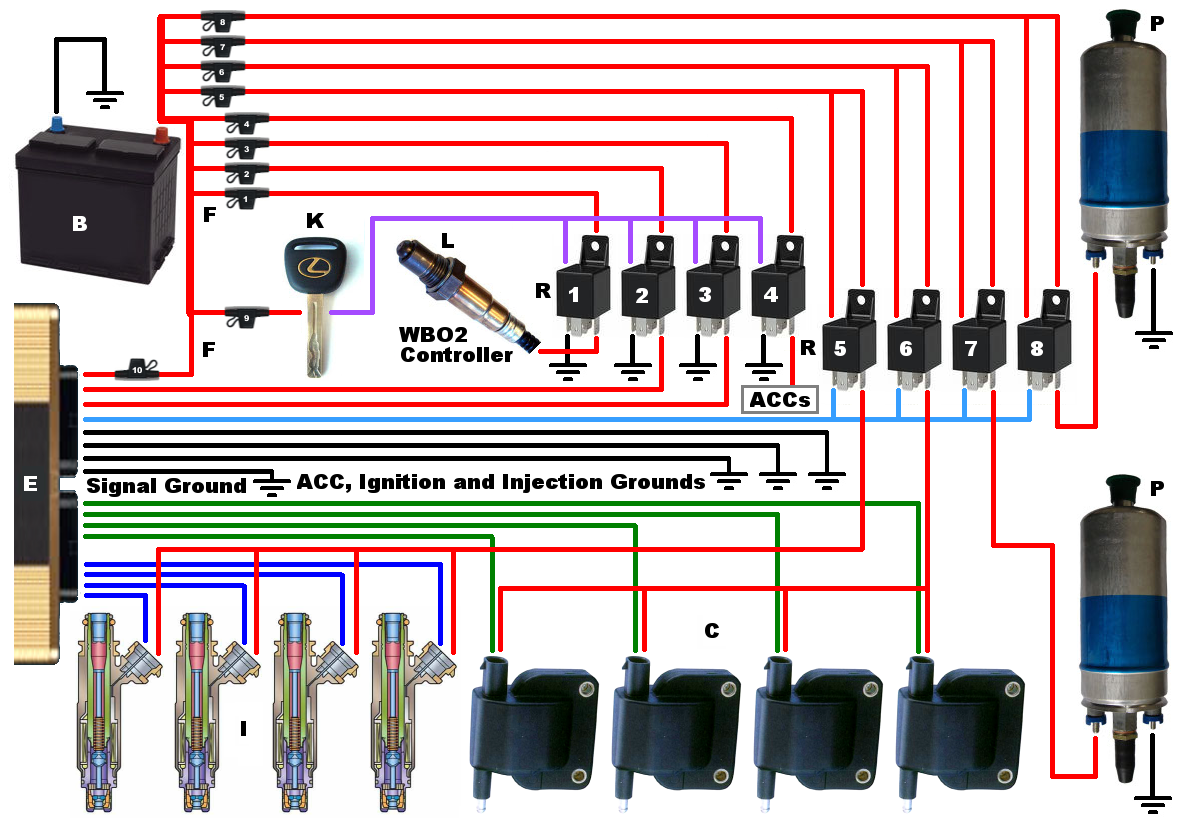
\includegraphics[width=1\textwidth]{images/freeems-power-wiring5.png}
\caption{Wiring diagram}
\label{fig:wiring}
\end{center}
\end{figure}

\subsection{Connector boards}
Puma is intended to have another board as an interface to the engine. This allows to have specific connectors and circuitry for some types of engines.

A connector boar template for Spin1 would look like this one:
\begin{center}
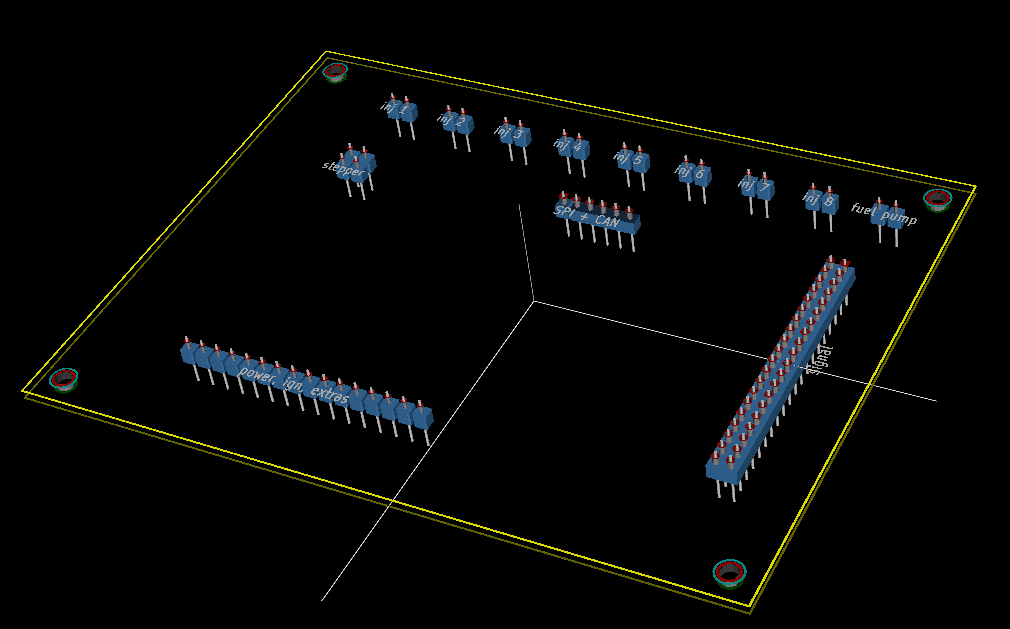
\includegraphics[width=0.8\textwidth]{images/connector_board3D.png}
\end{center}

If you don't have a Connector Board, you can design/make/buy your own, or just skip it and connect Puma directly to the engine.

\subsection{Puma's connections} %what a lame name

In case you want to connect the engine directly, or want to design a connector board, these are the connection layout of a Spin1 board:


\begin{figure}[h!]
\begin{center}
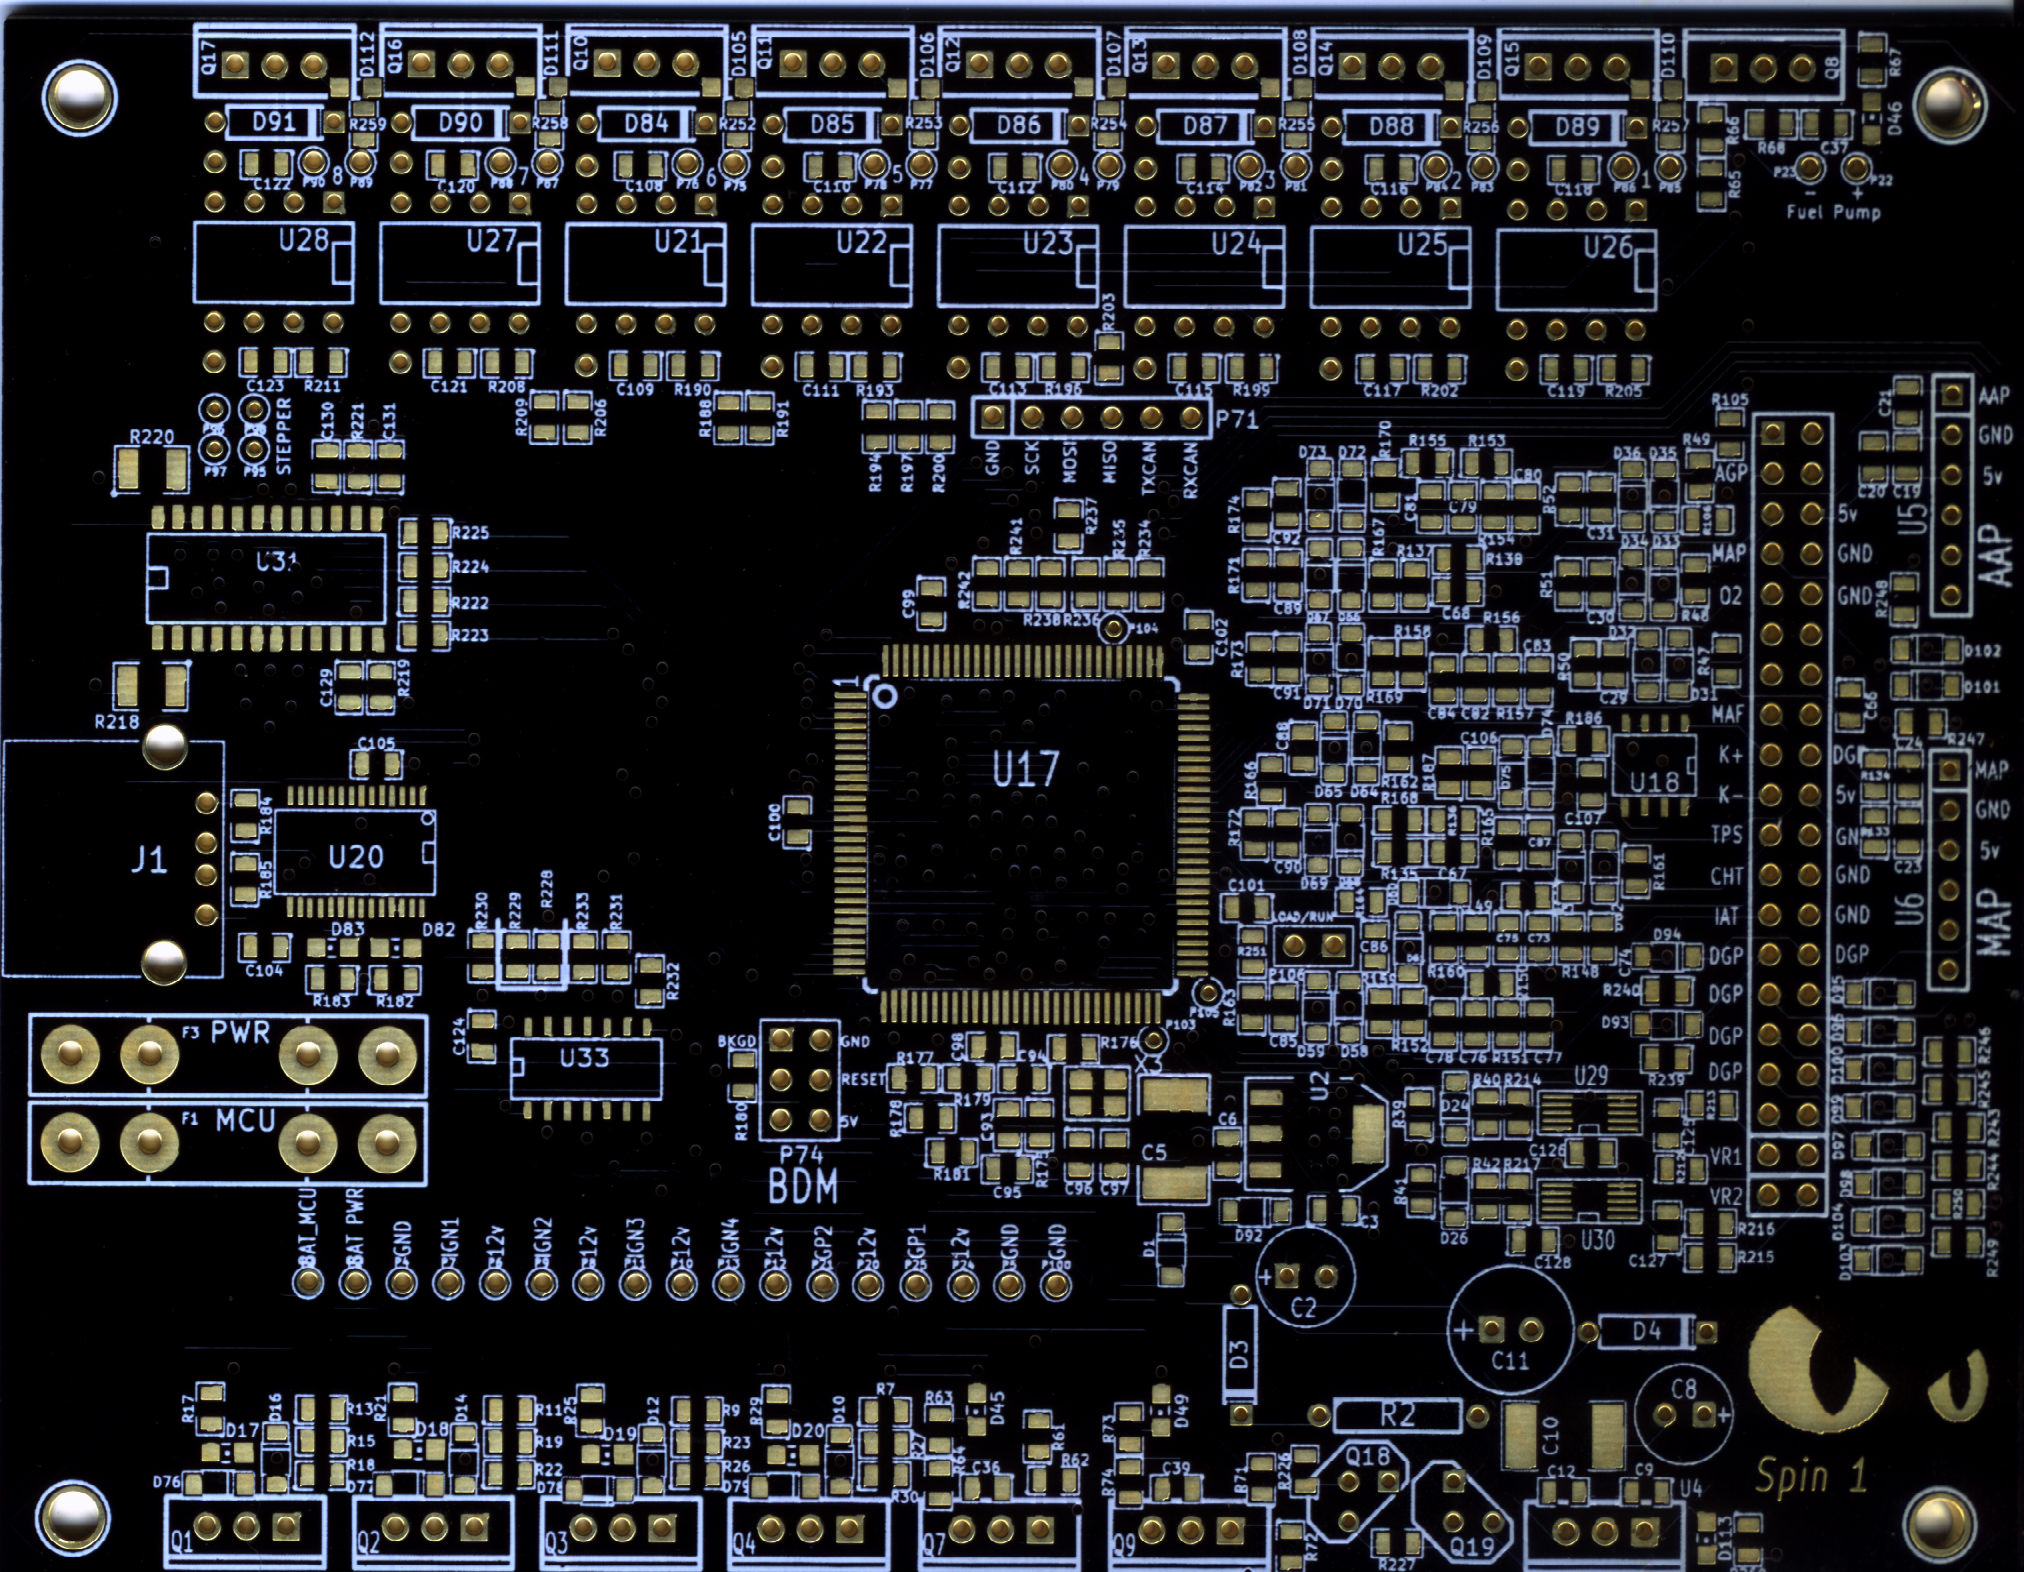
\includegraphics[width=1\textwidth]{images/Spin1_front.png}
\label{fig:Spin1_front}
\end{center}
\end{figure}

\begin{center}
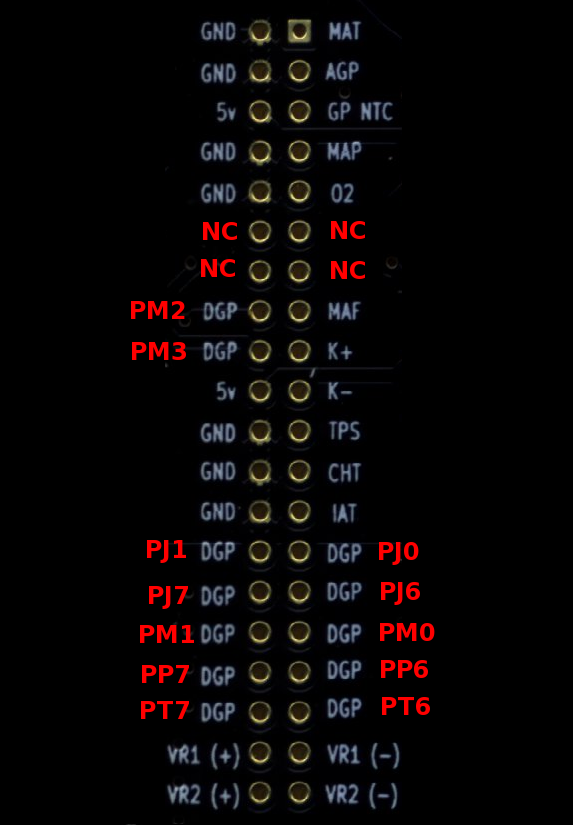
\includegraphics[width=0.4\textwidth]{images/PumaSpin1HeaderPinOut.png}
\end{center}

For digital crank/cam inputs, leave VR(-) floating and connect the signal wire to VR(+). It will set the treshold to 2.5v.

\subsection{Grounding}

Connect power grounds as noted in \ref{fig:Spin1_front}. This is the single most important part of the assembly

Don't make high currents go trough sensors ground, use at least 5(?) ground wires to the battery in your installation.

%insist on the grounding

\section{Troubleshooting}

You followed exactly what this document said, but things didn't worked well. Ok, fear not, lets do some basic checking:

\begin{itemize}
 \item FreeEMS code is loaded but it doesn't run.

Verify the firmware you loaded:
Open Loader-\textgreater Rip, and diff the .s19 file with the original. The only differences should be in the last part (that is the SM itself)

If it seems right, you are probably in Serial Monitor mode.

The LOAD/RUN header should be left open to allow for FreeEMS code to run. While in SM mode, the header pin is at 0v, and while running FreeEMS, the same pin has a ~50hz square wave (with a multimeter you'll measure 2.5v). %%Fred, is this normal or that was just noise triggering the tacho output?

The FT232 output (pin 1) must have a strong pullup so the MCU can leave the SM mode (point to USB hack), check it is working.

 \item Nothing works:

Check PLL and oscillator by measuring the voltage in the MCU-side of R175. It should be around 1.5v. If it is 2.5v (totally pulled up), you have a problem with the crystal or the PLL circuits. Check the solderings or continuity.
 \item BDM pod throws an error:

Check you have 5v or 2.5v in all the required VDD pins. Check continuity in the BKDM line. Check PLL and crystal.


\end{itemize}


\section{Spin1 specific notes}

\begin{enumerate}
\item This spin has several modifications. Start these modifications by cutting the wrong traces, and adding jumpers as shown below.

The FT232 IC needs also a pnp transisitor or it will make the mcu start always in SM mode.

If you want blinking leds for the usb, there is a pulldown that should be a pullup.

To begin your USB modifications, take reference from the following pictures:

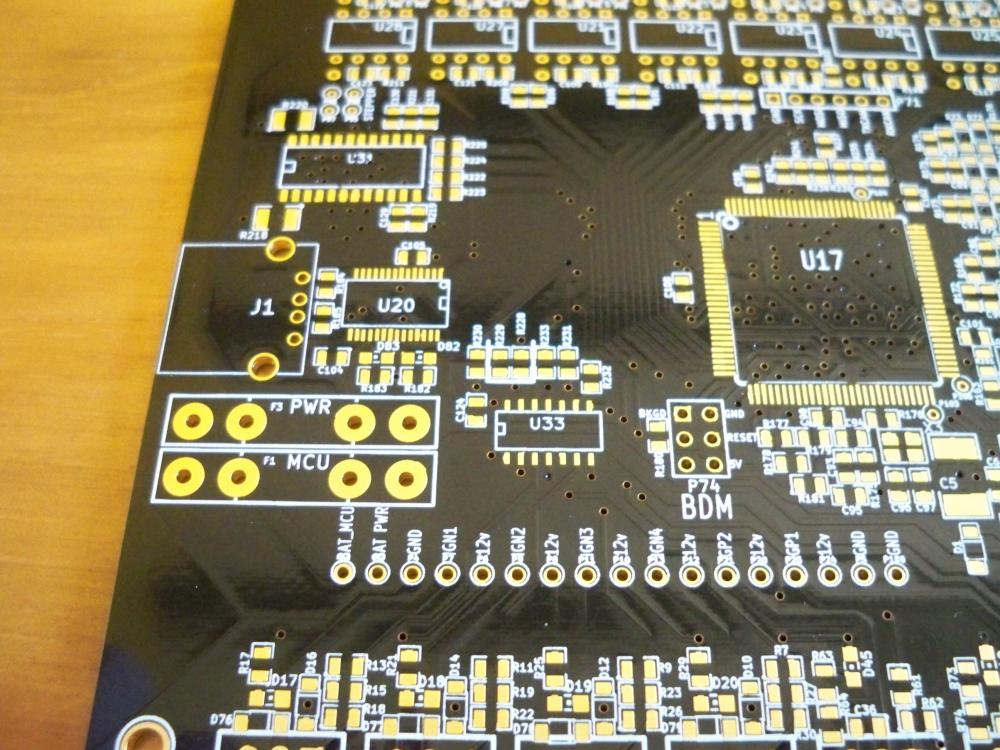
\includegraphics[width = 0.4\textwidth]{images/step1.jpg}
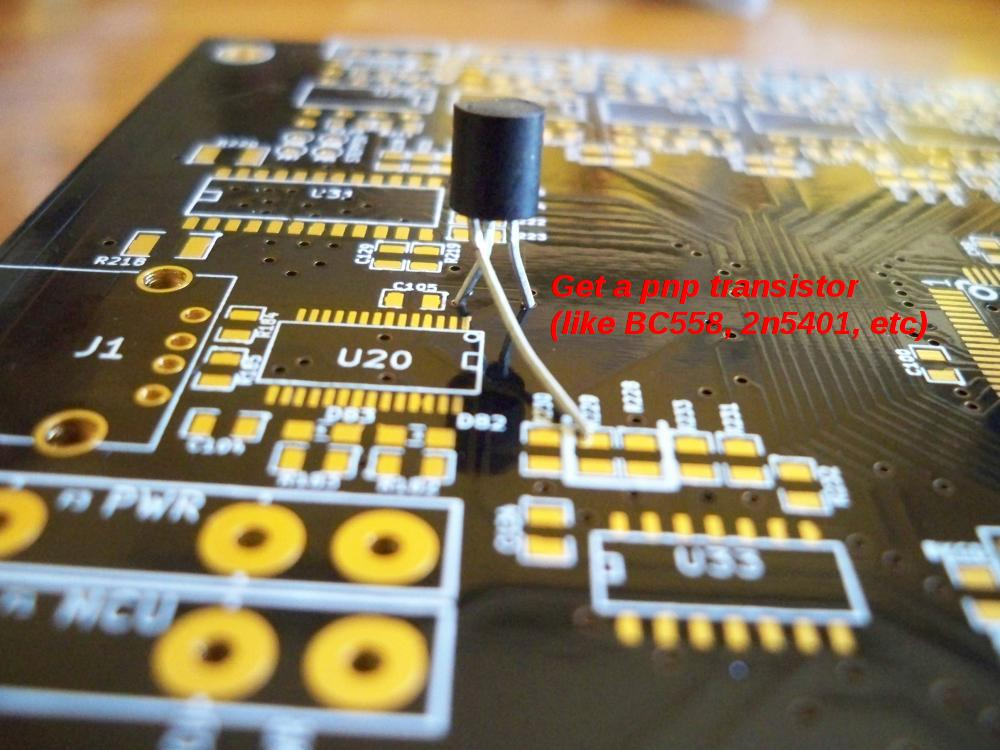
\includegraphics[width = 0.4\textwidth]{images/step2.jpg}

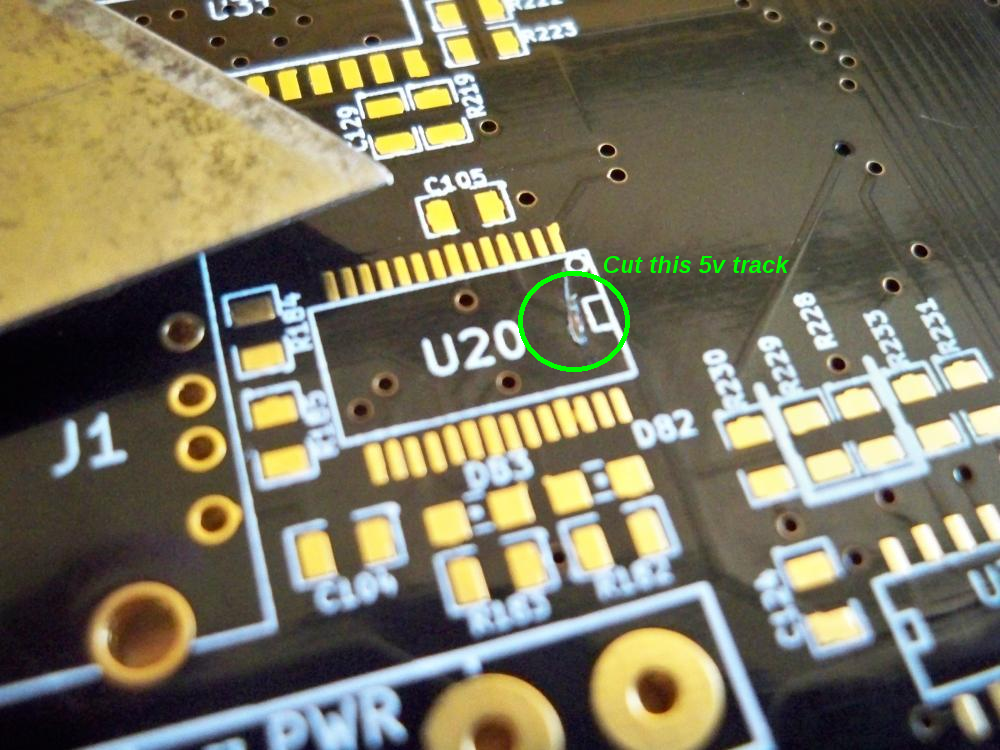
\includegraphics[width = 0.4\textwidth]{images/step4.png}
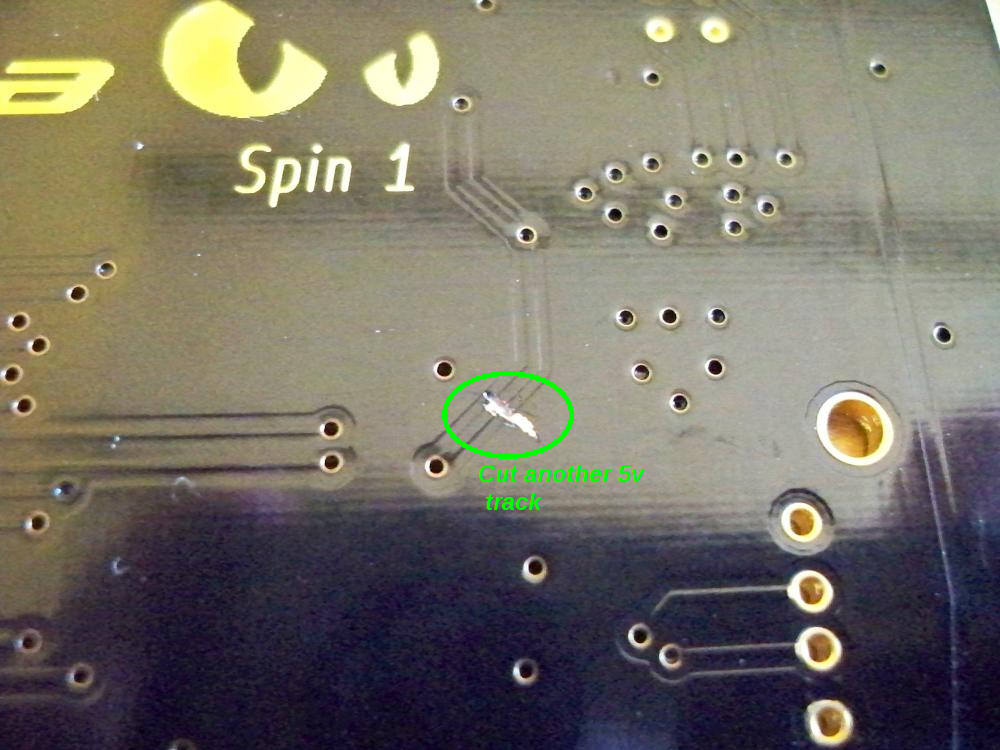
\includegraphics[width = 0.4\textwidth]{images/step5.png}

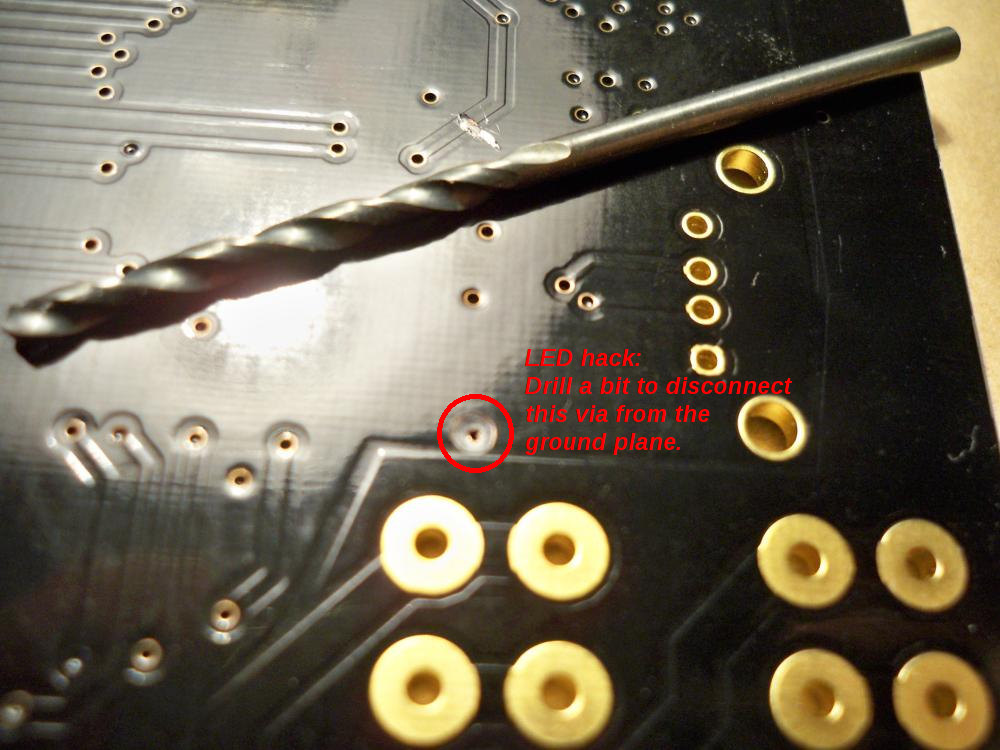
\includegraphics[width = 0.4\textwidth]{images/step6.png}
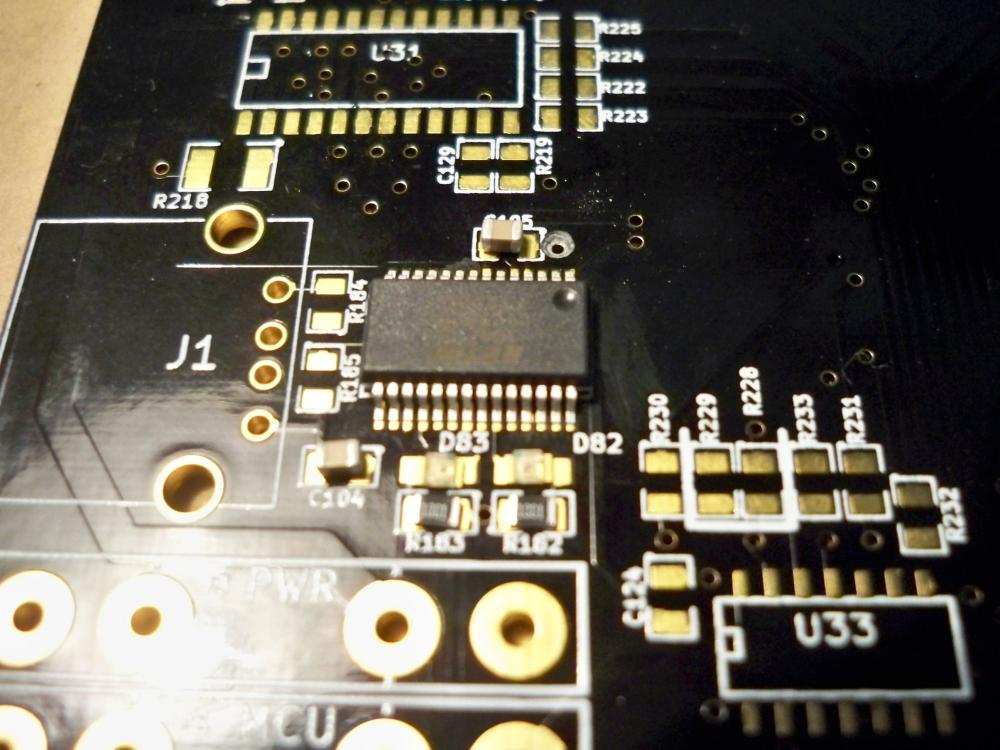
\includegraphics[width = 0.4\textwidth]{images/step7.jpg}

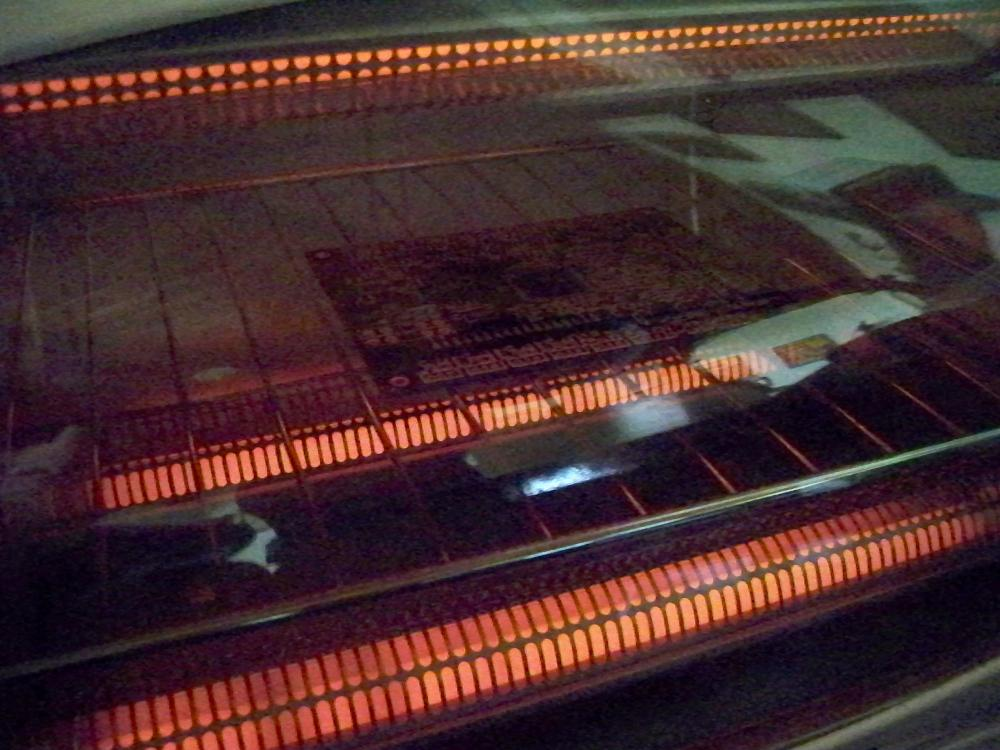
\includegraphics[width = 0.4\textwidth]{images/step8.jpg}
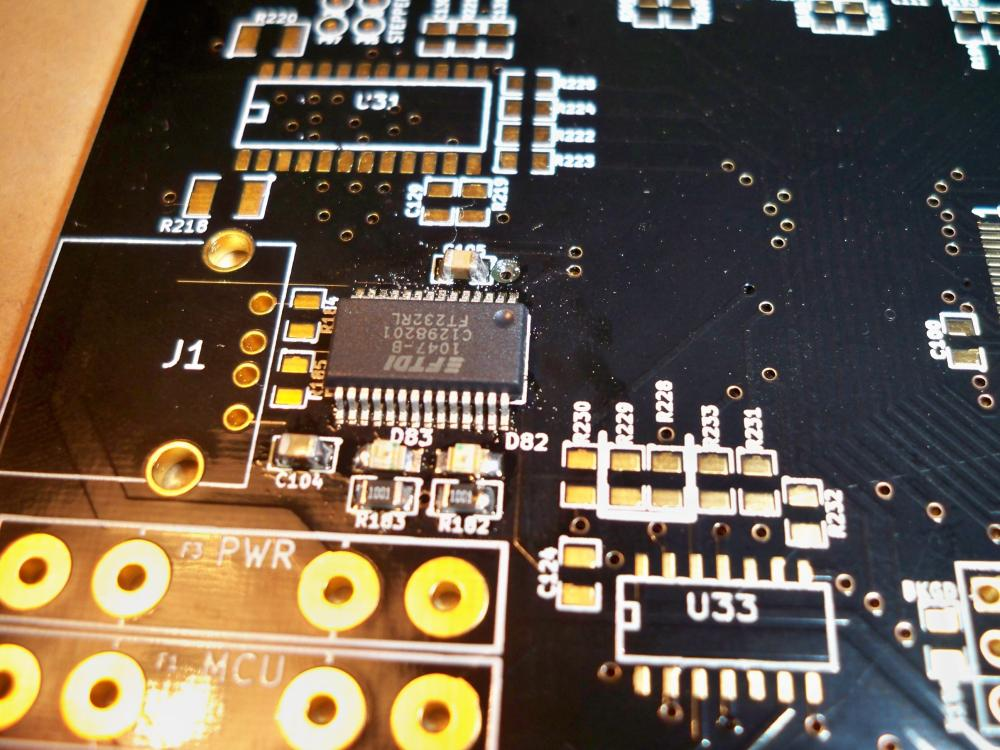
\includegraphics[width = 0.4\textwidth]{images/step9.jpg}

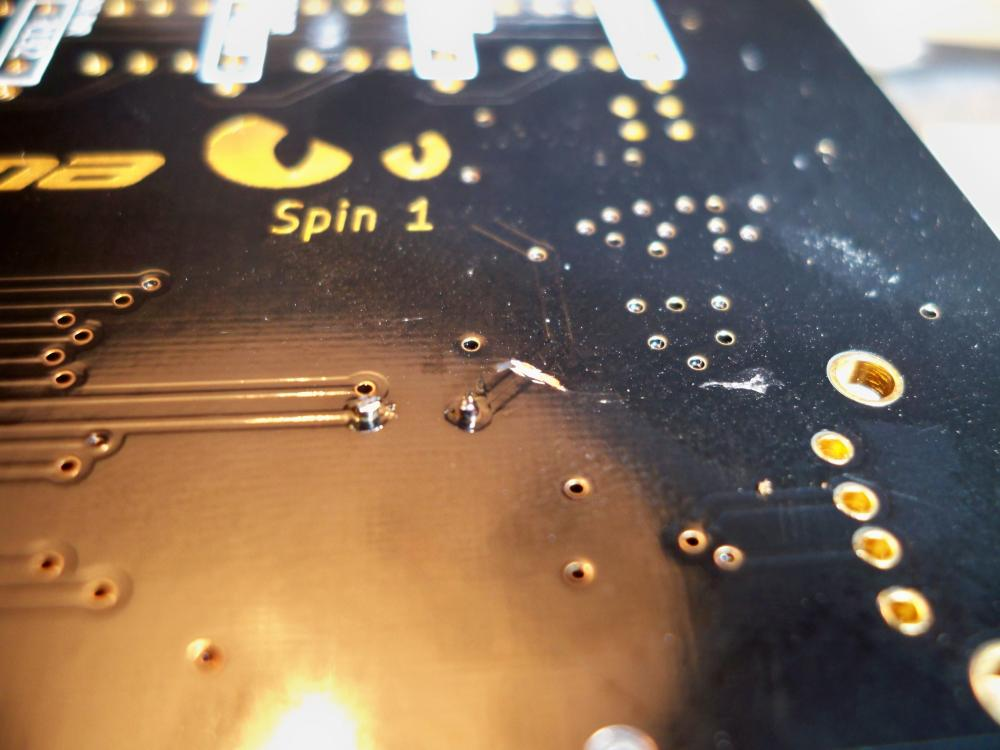
\includegraphics[width = 0.4\textwidth]{images/step10.jpg}
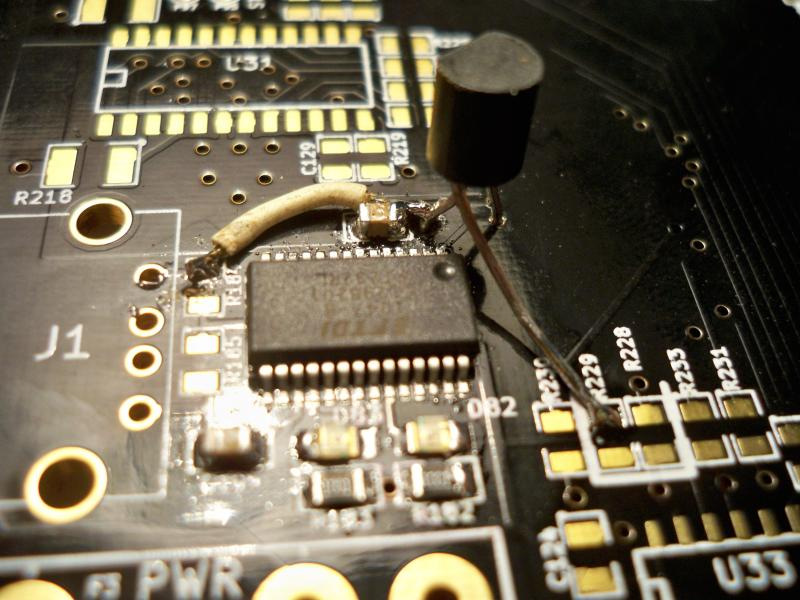
\includegraphics[width = 0.4\textwidth]{images/step11.jpg}

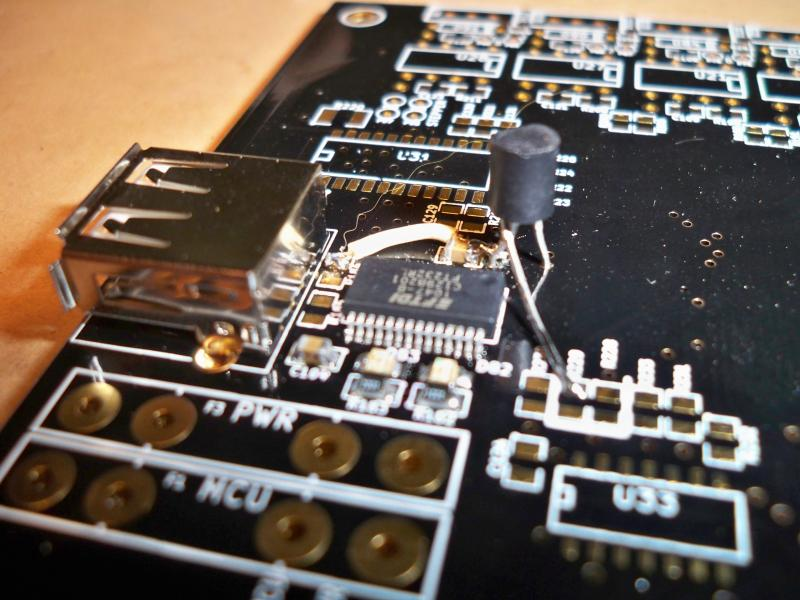
\includegraphics[width = 0.4\textwidth]{images/step12.jpg}
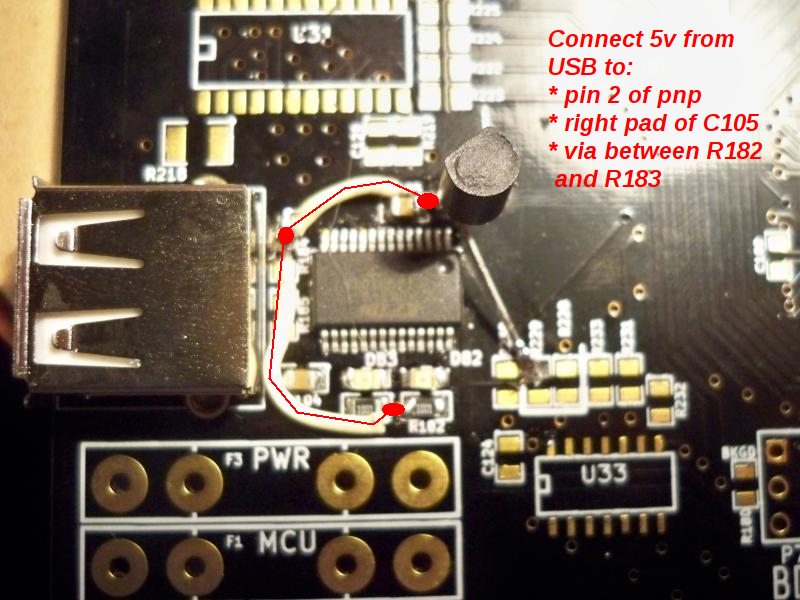
\includegraphics[width = 0.4\textwidth]{images/step13.png}

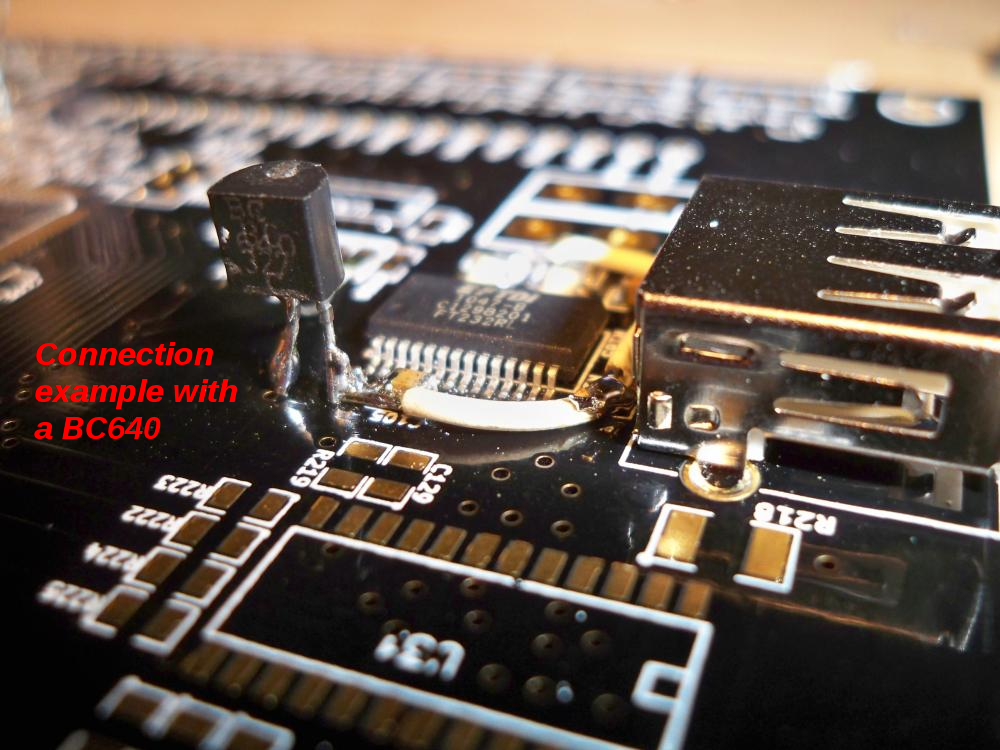
\includegraphics[width = 0.4\textwidth]{images/step14.png}
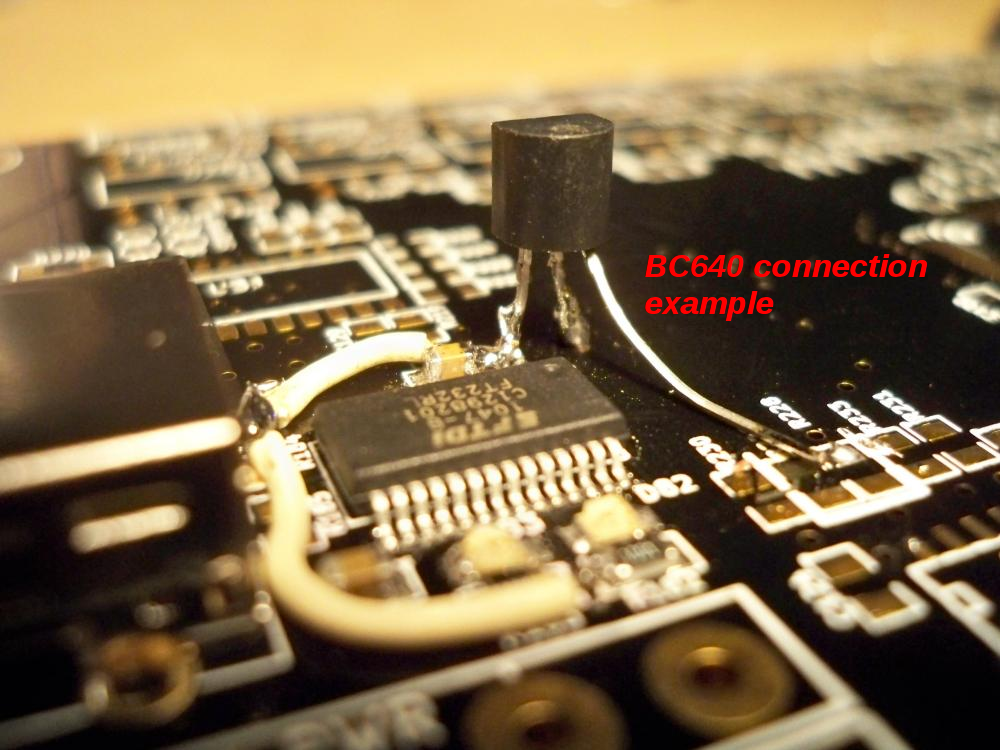
\includegraphics[width = 0.4\textwidth]{images/step15.png}

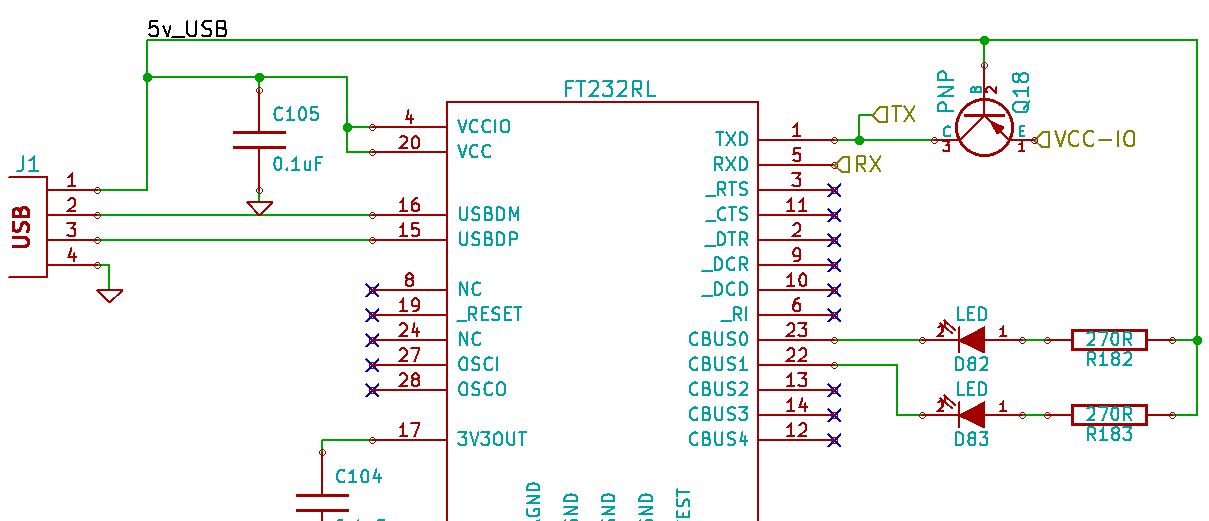
\includegraphics[width=0.95\textwidth]{images/FT232_sch.png}
\newline

If you're going to drive a high impedance injector, we suggest a VNP35N07, and here you can see how it is connected.

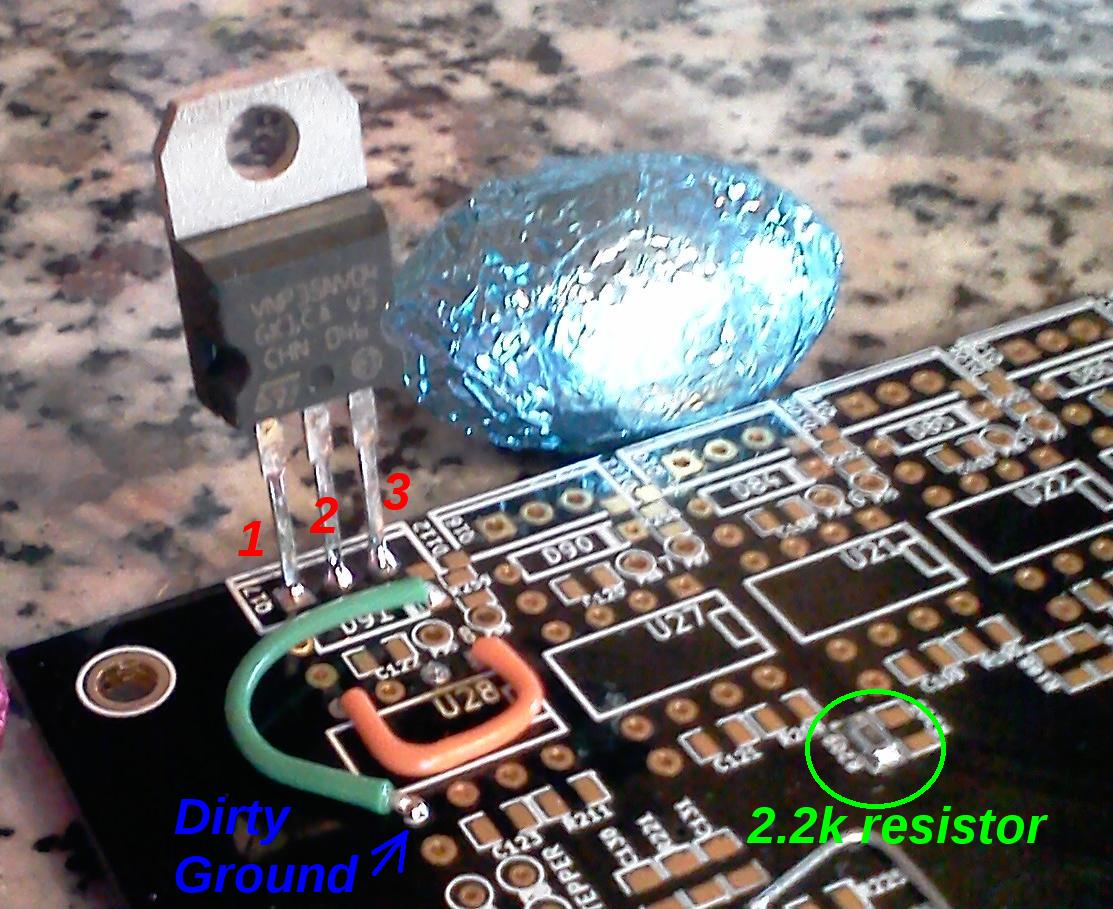
\includegraphics[width = 0.4\textwidth]{images/injector_hack_front.jpeg}
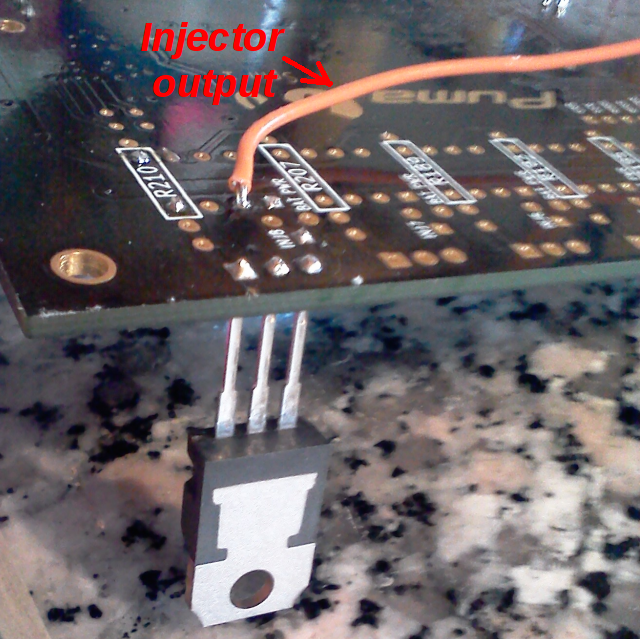
\includegraphics[width = 0.4\textwidth]{images/injector_hack_back.png}

Repeat as necessary if you need more than one injector output. The eight injector circuits are identical, the only moving target is the resistor between MCU and transistor gate, but you'll figure it out, they're in a similar position. Use a multimer if you have doubts, or just ask.

In this particular logic input fet, pin 1 is the input, pin 2 the drain, and pin 3 the source. If you have other pinout, ask for a suggestion and please share pictures of it. Also, you can check directly the kicad files to decide where to put bridges (sharing pictures would be cool too).
\newline



\begin{figure}[htb]
  \centering
  \subfigure[Cut wrong VDD traces]{
  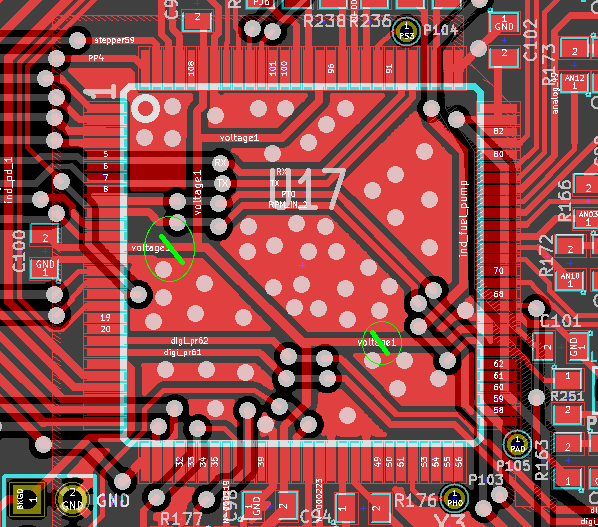
\includegraphics[width=0.45\textwidth]{images/MCU_VDD_traces.png}
  \label{fig:mcu_traces}
  }
  \subfigure[Correct the BRV source, it shoud come directly from the battery to the via next to R105]{
  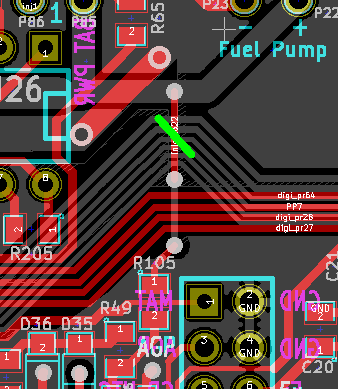
\includegraphics[width=0.45\textwidth]{images/BRV_hack.png}
  \label{fig:brv_hack}
  }
  \subfigure[FT232 circuit -lacks PNP-!!]{
  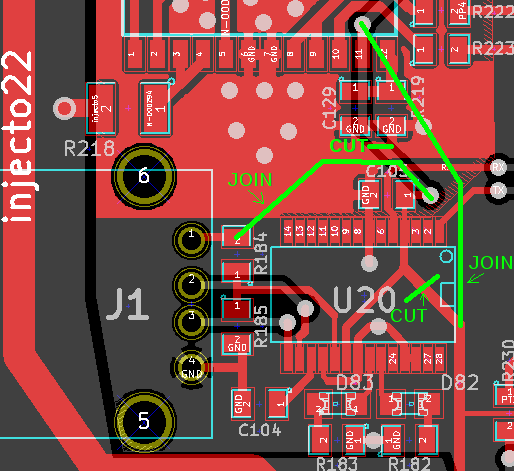
\includegraphics[width=0.45\textwidth]{images/USB_power_hack.png}
  \label{fig:usb_hack}
  }
  \caption{Spin1 mods}
\end{figure}

\item You have the PCB + components, so get KICAD and the files, or the pdf files from puma.freeems.org. PDFs aren't search-able so you may want to choose to install KICAD until we workout that.

\item Start the assembly!

Just solder the components. If you ordered a board, you should know how to do it. An oven is a fast way to get it done.

Don't put too much paste for the small regulator, or it will get misaligned.

Components that shouldn't be populated:

\begin{itemize}
\item F1, F3 (Fuses)
\item R226, R227, Q18, Q19, bridge pin 1 and 3 of Q19 (this is the shutdown circuit)
\item R133 (bad pullup)
\item R228 OR R229, using one of them defines whether the XOR negates or not its outputs.
\item If you use VR inputs, R212, R213, R215, and R216 should be bigger, like $\frac{1}{4}$ or $\frac{1}{2}$W. 10k\ohm to 20k\ohm will be fine.
\item U18, R186, R187, C107, D74, D75, C106 (thermocouple driver)
\end{itemize}

\item Program the MCU using a BDM pod.

Install Codewarrior, open the programmer, go to File $\rightarrow$ Load application, and select the .s12 (FreeEMS serial monitor).

It should get connected, program it, verify, and never complain.

\item Load FreeEMS firmware, using seank's loader.

\item Install MTX and connect to the board to the PC to check that freeems is running.

\end{enumerate}



\end{document}


